%\documentclass[preprint,prl,superscriptaddress]{revtex4-1}
%\documentclass[twocolumn,nofootinbib]{nature}
\documentclass[onecolumn,pra,superscriptaddress,nofootinbib]{revtex4-1}

% packages
\usepackage[dvips]{graphicx} % for figures
\usepackage{amsfonts,amssymb,amscd,amsmath,amsthm}
\usepackage{textcomp}
\usepackage{enumerate}
\usepackage{epsfig}
\usepackage{subfigure}
\usepackage{xcolor}
%\usepackage[expert]{mathdesign}

\newcommand{\bra}[1]{\mbox{$\left\langle #1 \right|$}}
\newcommand{\ket}[1]{\mbox{$\left| #1 \right\rangle$}}
\newcommand{\braket}[2]{\mbox{$\left\langle #1 | #2 \right\rangle$}}

\newtheorem{theorem}{Theorem}
\newtheorem{lemma}{Lemma}
\newtheorem{corollary}{Corollary}
\newtheorem{claim}{Claim}
\newtheorem{conjecture}{Conjecture}
\newtheorem*{observation}{Observation}
\newtheorem{definition}{Definition}

\begin{document}

\title{Lecture 1: one-qubit system}

%% For REVTeX it is possible to automate superscript and e-mail callouts with the superscriptaddress option; see REVTeX4 documentation.


\author{Xiongfeng Ma}
\email{xma@tsinghua.edu.cn}
\affiliation{Center for Quantum Information, Institute for Interdisciplinary Information Sciences, Tsinghua University, Beijing 100084, China}


\begin{abstract}
In this chapter, we shall learn about the simplest system in quantum information --- qubit. A qubit can be represented by a quantum state, processed by operators, and read out by measurement. Here, we focus on one qubit system: pure state, projection-valued measure (PVM), and unitary transformation. We shall also cover some related concepts: Born's law, density matrix, Bloch sphere, Pauli matrices, quantum no-cloning theorem, no-deletion theorem.
\end{abstract}

%\ocis{(270.5565) Quantum communications; (270.5568) Quantum cryptography.}


\maketitle %% required


\section{Notations and definitions}
A state is a complete description of a physical system.

\subsection{Dirac's bra-ket notations}
\begin{enumerate}
\item
Ket: $\ket{\psi}$ denotes a quantum state $\psi$, $\ket{0}$ denotes $\begin{pmatrix}1\\0\end{pmatrix}$ and $\ket{1}$ denotes $\begin{pmatrix}0\\1\end{pmatrix}$.
\begin{equation} \label{ket}
\begin{aligned}
\psi &= \begin{pmatrix}a\\b\end{pmatrix}=a\begin{pmatrix}1\\0\end{pmatrix} + b\begin{pmatrix}0\\1\end{pmatrix} \\
\ket{\psi} &= a\ket{0}+b\ket{1},
\end{aligned}
\end{equation}
where $a, b\in\mathcal{C}$.

\item
Bra: $\bra{\psi}$ denotes $\psi^\dag$, the Hermitian conjugate of $\ket{\psi}$, $\bra{0}$ denotes $(1,0)$ and $\bra{1}$ denotes $(0,1)$.
\begin{equation} \label{bra}
\begin{aligned}
\psi^\dag &= \begin{pmatrix}a^* &b^*\end{pmatrix}=a^*\begin{pmatrix}1 &0\end{pmatrix}+b^*\begin{pmatrix}0 &1\end{pmatrix} \\
\bra{\psi} &= a^*\bra{0}+b^*\bra{1},
\end{aligned}
\end{equation}


\item
Inner~ product of two quantum states
\begin{equation} \label{inner product }
\begin{aligned}
\braket{\psi_1}{\psi_2}=\begin{pmatrix}a^*_1 &b^*_1\end{pmatrix} \begin{pmatrix}a_2\\b_2\end{pmatrix} =a^*_1a_2+b^*_1b_2.\\
\end{aligned}
\end{equation}
\end{enumerate}


\subsection{Hilbert space}
Quantum states form a Hilbert space $\mathcal{H}$.  A Hilbert space is a vector space (with an inner product) over the complex numbers $\mathcal{C}$. Vectors will be denoted $\ket{\psi}$ (Dirac's bra-ket notation). In quantum mechanics, a state is a ray in a Hilbert space. A Hilbert space has the properties:
\begin{enumerate}[i)]
\item
Positivity: $\braket{\psi}{\psi}>0$ for $\ket{\psi}\ne0$.
\item
Linearity: $\bra{\phi}(a\ket{\psi_1})+b\ket{\psi_2})=a\braket{\phi}{\psi_1}+b\braket{\phi}{\psi_2}$.
\item
Skew symmetry: $\braket{\phi}{\psi}=\braket{\psi}{\phi}^*$.
\end{enumerate}


\subsection{ray}
\begin{enumerate}[$\cdot$]
\item It is an equivalence class of vectors that differ by
multiplication by a nonzero complex scalar.
\item For any nonzero ray, we can by convention choose a representative of the class, denoted $\ket{\psi}$, that has
unit norm:

\begin{equation} \label{ray}
\begin{aligned}
\braket{\psi}{\psi}=1.\\
\end{aligned}
\end{equation}
\item Thus states correspond to normalized vectors, and the overall phase of
the vector has no physical significance:$\ket{\psi}$ and $e^{i\alpha}\ket{\psi}$ describe the same
state, where $|e^{i\alpha}|=1$.
\item Since every ray corresponds to a possible state, given two states $\ket{\phi}$, $\ket{\psi}$,
another state can be constructed as the linear superposition of the two, $a\ket{\phi}+b\ket{\psi}$.
The relative phase in this superposition is physically significant.
\item We identify $a\ket{\phi}+b\ket{\psi}$ with $e^{i\alpha}(a\ket{\phi}+b\ket{\psi})$ but not with
$a\ket{\phi}+e^{i\alpha}b\ket{\psi}$.
\end{enumerate}



\section{A pure qubit}
A bit in information theory can be represented by 0/1, which could be used to represent two states of a capacitor --- high/low voltage. We assume these two states 0/1 can be unambiguously distinguished.

A qubit is an analogy of bit. Similarly, a qubit represents the state of a two-level system  by a ket $\ket{0}$ and $\ket{1}$. The difference is that a qubit can be prepared in a superposition of the two states $\ket{0}$ and $\ket{1}$, which is indicated as a linear combination of the two states. If the two states $\ket{0}$ and $\ket{1}$ can be treated as two orthogonal vectors,
\begin{equation} \label{Qubit:purequbits}
\begin{aligned}
\ket{\phi}=a\ket{0}+b\ket{1},\\
\end{aligned}
\end{equation}
where $a,b\in \mathcal{C}$. Notes on the state representation:
\begin{enumerate}
\item
Born's probability interpretation: if one measures\footnote{Very soon, we shall learn how to do ``measure".} the state Eq.~\eqref{Qubit:purequbits}, there is a probability $|a|^2/(|a|^2+|b|^2)$ to get 0 and a probability $|b|^2/(|a|^2+|b|^2)$ to get 1.

\item
From Born's law, the overall factor in Eq.~\eqref{Qubit:purequbits}, $|a|^2+|b|^2$, does not affect the state. One can pick $|a|^2+|b|^2=1$ as normalized state representation.

\item
Strictly speaking, $\ket{\phi}$ represents a \emph{ray} instead of a vector, same for $\ket{0}$ and $\ket{1}$.

\item
The outcome is intrinsically random according Born's law. Einstein, ``God does not play dice with the universe". In fact, we can experimentally verify this\footnote{Later, we shall cover this in Bell's inequality. You are encouraged to read more interesting materials on the debate between Einstein and Bohr.}!
\end{enumerate}

Define density matrix of a quantum state,
\begin{equation} \label{Qubit:densitymat}
\begin{aligned}
\rho &=\ket{\phi}\bra{\phi} \\
&=(a\ket{0}+b\ket{1})(a^*\bra{0}+b^*\bra{1}) \\
&= |a|^2\ket{0}\bra{0}+|b|^2\ket{1}\bra{1}+ab^*\ket{0}\bra{1}+a^*b\ket{1}\bra{0} \\
&= \begin{pmatrix} |a|^2 & ab^* \\ a^*b & |b|^2\end{pmatrix}.
\end{aligned}
\end{equation}
A density matrix (of a pure qubit) has following properties:
\begin{enumerate}
\item
self-adjoint: $\rho^\dag=\rho$

\item
trace one: $Tr(\rho)=1$

\item
positivity: $\rho\ge0$

\item
*$\rho^2=\rho$
\end{enumerate}

Question: Born's law is reflected in the diagonal terms of Eq.~\eqref{Qubit:densitymat}. Are the off-diagonal terms useless?


\subsection{Bloch sphere}
When $a, b$ are real numbers, the state in Eq.~\eqref{Qubit:purequbits} can be represented by rays in $x$-$y$ plane. Of course, for any state such that $a/b$ or $b/a$ is a real number, the rays form a plane. What if $a, b$ are general complex numbers? We need to think how many free (real) parameters existing in Eq.~\eqref{Qubit:purequbits}. Since $|a|^2+|b|^2$ does not affect the state, we can always set it to be 1 (normalized state representation). Thus, there are two free (real) parameters.

A normalized pure state of a qubit can be written as
\begin{equation} \label{eq:BlochSphere}
\begin{aligned}
\ket{u} = \cos\frac{\theta}{2}\ket{0}+e^{i\varphi}\sin\frac{\theta}{2}\ket{1}.
\end{aligned}
\end{equation}
Therefore, it is convenient to represent it as a vector living the surface of a unit sphere with the spherical coordinate $(r=1,\theta,\varphi)$.

\begin{figure}[tbh]
\centering \resizebox{6cm}{!}{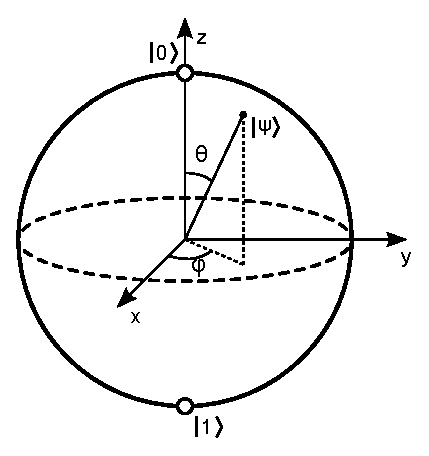
\includegraphics{epsBlochSphere.eps}}
\caption{Bloch sphere.} \label{fig:BlochSphere}
\end{figure}

Exercise: write down the states of $\ket{x+}$, $\ket{x-}$, $\ket{y+}$, $\ket{y-}$, $\ket{z+}$, $\ket{z-}$, according to Eq.~\eqref{eq:BlochSphere}.

Question: how a pair of orthogonal qubits represented in the Bloch sphere?

\subsection{Pauli matrix and qubit basis}
Pauli matrices are a set of three $2\times2$ complex matrices which are Hermitian unitary,
\begin{equation} \label{eq:PauliMatrix}
\begin{aligned}
\sigma_x &=
    \begin{pmatrix}
      0&1\\
      1&0
    \end{pmatrix}, \quad\quad
\sigma_y &=
    \begin{pmatrix}
      0&-i\\
      i&0
    \end{pmatrix}, \quad\quad
\sigma_z &=
    \begin{pmatrix}
      1&0\\
      0&-1
    \end{pmatrix}.
\end{aligned}
\end{equation}
For those who are interested in where these Pauli matrices come from, you are encouraged to read Chapter 2 of John Preskill's lecture notes.

\begin{equation} \label{eq:IPauliVector}
\begin{aligned}
\sigma_0 &=
    \begin{pmatrix}
      1&0\\
      0&1
    \end{pmatrix}, \quad\quad
\vec{\sigma} &= (\sigma_x,\sigma_y,\sigma_z)
\end{aligned}
\end{equation}


A qubit can be prepared in three bases: $X$, $Y$, $Z$, which are corresponding to the eigenstates of Pauli matrices: $\sigma_x$, $\sigma_y$, $\sigma_z$, respectively. Denote the eigenstates of the $Z$ basis by $\ket{0}$ and $\ket{1}$, then the other eigenstates of the $X$ and $Y$ bases are
\begin{equation} \label{eq:XYZbasis}
\begin{aligned}
\ket{\pm} &= (\ket{0}\pm\ket{1})/\sqrt2, \\
\ket{\pm i} &= (\ket{0}\pm i\ket{1})/\sqrt2, \\
\end{aligned}
\end{equation}
respectively. These three bases are mutually unbiased bases (MUB), that is,
\begin{equation} \label{eq:MUB}
\begin{aligned}
\braket{\psi_i}{\phi_j} &= 1/\sqrt d, \\
\end{aligned}
\end{equation}
where $\ket{\psi_i}$ and $\ket{\phi_j}$ are basis states from two different MUB and $d$ is the dimension.


\subsection{Qubit tomography}
In general, a qubit might be in a mixed state, and then it will be within the Bloch sphere instead on the surface. In general, the density matrix of a qubit can be written as
\begin{equation} \label{eq:rhoBloch}
\begin{aligned}
\rho &= \frac12(\sigma_0+\vec{P}\cdot \vec{\sigma}) \\
&= \frac12
    \begin{pmatrix}
      1+P_z&P_x-iP_y\\
      P_x+iP_y&1-P_z
    \end{pmatrix}
\end{aligned}
\end{equation}
where $\vec{P}=(P_x,P_y,P_z)$ is a vector and $|\vec{P}|\le1$. When $|\vec{P}|=1$, Eq.~\eqref{eq:rhoBloch} represents a pure qubit.

Quantum state tomography is the process of reconstructing the quantum state for a quantum system by proper measurements. The quantum state can be pure (vector) or in general mixed (density matrix). A set of measurements is called tomographically complete if it can uniquely identify the state. That is, the measurement outcomes are able to provide all the information about the state. In the classical physics, it corresponds to system calibration.

Let us take qubit tomography for example. As given in Eq.~\eqref{eq:rhoBloch}, the $Z$ basis measure provides the information on $P_z$. From Eq.~\eqref{eq:xzHadamard}, we know that the $X$ basis measure provides the information on $P_x$. Similarly, the $Y$ basis measure provides the information on $P_y$. Thus, $X$, $Y$, and $Z$ measurements is tomographically complete for a qubit. Another way to put this is,
\begin{equation} \label{eq:rho2tomo}
\begin{aligned}
\rho &= \frac12[tr(\rho)\sigma_0+tr(\sigma_x\rho)\sigma_x+tr(\sigma_y\rho)\sigma_y+tr(\sigma_z\rho)\sigma_z]. \\
\end{aligned}
\end{equation}
Now, let us move a bit further, tomography for $n$ qubits,
\begin{equation} \label{eq:rhontomo}
\begin{aligned}
\rho &= 2^{-n}\sum_{v_1,v_2,\dots,v_n\in\{0,x,y,z\}}tr(\sigma_{v1}\otimes\sigma_{v2}\otimes\cdots\otimes\sigma_{vn}\rho) \sigma_{v1}\otimes\sigma_{v2}\otimes\cdots\otimes\sigma_{vn},
\end{aligned}
\end{equation}
where the sum is over all possible the identity and Pauli matrices.

In another related concept, quantum process tomography, known quantum states are used to probe a quantum process to find out how the process can be described. Similarly, quantum measurement tomography works to find out what measurement is being performed.

The general principle behind quantum state tomography is that by repeatedly performing many different measurements on quantum systems described by identical density matrices, frequency counts can be used to infer probabilities, and these probabilities are combined with Born's rule to determine a density matrix which fits the best with the observations.




\section{Measurement}
Physics is an experimental science. If we observe (or measure) a quantum state in lab, what kind of outcomes do we expect and how are they related to the quantum state?

A measurement is a process in which information about the state of a physical system is acquired by an observer. In quantum mechanics, the measurement of an observable $A$ prepares an eigenstate of $A$, and the observer learns the value of the corresponding eigenvalue.

\subsection{Observables}
An observable is a self-adjoint operator on $\mathcal{H}$:
an observable is a property of a physical system that in principle can be measured. In quantum mechanics,
an observable is a self-adjoint operator.
\begin{enumerate}
\item
Operator: An operator is a linear map taking vectors to vectors,
\begin{equation} \label{operator}
\begin{aligned}
A:\ket{\psi}\mapsto A\ket{\psi},A(a\ket{\phi}+b\ket{\psi})=aA\ket{\phi}+bA\ket{\psi}.
\end{aligned}
\end{equation}

\item
Adjoint: The adjoint $A^\dag$ of the operator $A$ is defined by
\begin{equation} \label{adjoint}
\begin{aligned}
\braket{\psi}{A\phi}=\braket{A^\dag\psi}{\phi},
\end{aligned}
\end{equation}
for all vectors $\ket{\psi}$, $\ket{\phi}$.

\item
Self-adjoint: $A$ is self-adjoint if $A = A^\dag$, or in other words, if $\bra{\psi}A\ket{\phi}=\bra{\phi}A\ket{\psi}$ for all vectors $\ket{\psi}$, $\ket{\phi}$.
\begin{enumerate}[i)]
\item If $A$ and $B$ are self adjoint, then so is $A+B$ (because $(A + B)^\dag = A^\dag + B\dag$).
\item $(AB)^\dag = B^\dag A^\dag$, so that $AB$ is self adjoint only if $A$ and $B$ commute.
\item Note that $AB + BA$ and $i(AB ?- BA)$ are
always self-adjoint if $A$ and $B$ are.
\end{enumerate}

\item
A self-adjoint operator in a Hilbert space H has a spectral representation-its eigenstates form a complete orthonormal basis in $\mathcal{H}$.
We can express a self-adjoint operator $A$ as
\begin{equation} \label{self-adjoint operator}
\begin{aligned}
A=\sum_{n}a_nE_n.\\
\end{aligned}
\end{equation}
Here each $a_n$ is an eigenvalue of $A$, and $E_n$ is the corresponding orthogonal projection onto the space of eigenvectors with eigenvalue $a_n$. The
$E_n$ is satisfy,

\begin{equation} \label{eigenvectors}
\begin{aligned}
E_nE_m=\delta_{n,m}E_n,\\
E_n^\dag=E_n.\\
\end{aligned}
\end{equation}

\item
The orthogonal projector onto the one-dimensional space spanned by the vector $\ket{\psi}$ may be expressed as $\ket{\psi}\bra{\psi}$, where $\bra{\psi}$ is the bra that annihilates
vectors orthogonal to $\ket{\psi}$. Therefore, an alternative notation for the spectral representation of $A$ is
 \begin{equation} \label{spectral representation}
\begin{aligned}
A=\sum_n\ket{n}a_n\bra{n},\\
\end{aligned}
\end{equation}
where $\{\ket{n}\}$ is the orthonormal basis of eigenstates of $A$, with $A\ket{n} =a_n\ket{n}$.

\end{enumerate}




\subsection{Projection-valued measure}
A projection-valued measure (PVM) is an orthogonal projection.

\begin{enumerate}
\item
If the quantum state just prior to the measurement is $\ket{\psi}$, then the outcome an is obtained
with a priori probability,
\begin{equation} \label{priori probability}
\begin{aligned}
\mathbf{Prob}(a_n)=||E_n\ket{\psi}||^2=\bra{\psi}E_n\ket{\psi}.
\end{aligned}
\end{equation}
\item if the outcome $a_n$ is attained, then the (normalized) quantum state
just after the measurement is
\begin{equation} \label{State after measurement}
\begin{aligned}
\frac{E_n\ket{\psi}}{||E_n\ket{\psi}||}.\\
\end{aligned}
\end{equation}

\item
If the measurement is immediately repeated, then according to this rule the same outcome is obtained again, with probability one.

\item
If many identically prepared systems are measured, each described by the state $\ket{\psi}$,
then the expectation value of the outcomes is,
\begin{equation} \label{expectation value}
\begin{aligned}
\langle a\rangle\equiv\sum_{n}a_n\mathbf{Prob}(a_n)=\sum_{n}\bra{\psi}E_n\ket{\psi}=\bra{\psi}A\ket{\psi}.\\
\end{aligned}
\end{equation}

\end{enumerate}




\section{Unitary transformation}
In quantum mechanics, the state evolution through time follows Schrodinger's equation, shown in Fig.~\ref{fig:SchrodingerEq}. For the moment, we do not want to going to any details for the equation. All we need to know is that the evolution is unitary.

\begin{figure}[tbh]
\centering \resizebox{8cm}{!}{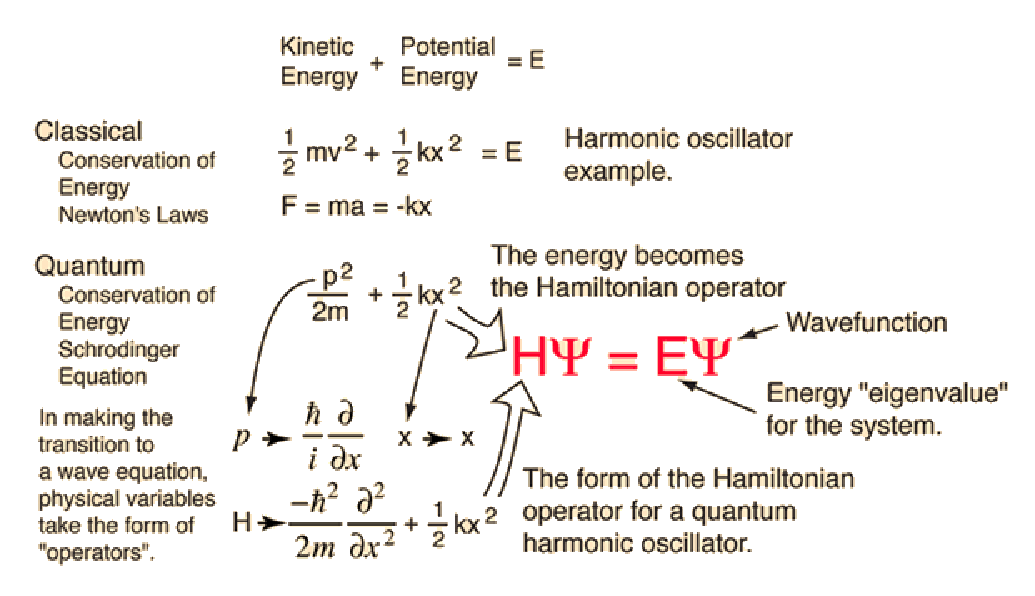
\includegraphics{epsSchEq.eps}}
\caption{Schrodinger's equation} \label{fig:SchrodingerEq}
\end{figure}

A widely used single qubit operation, Hadamard transformation,
\begin{equation} \label{eq:Hadamard}
\begin{aligned}
H &= \frac{1}{\sqrt2}
    \begin{pmatrix}
      1&1\\
      1&-1
    \end{pmatrix},
\end{aligned}
\end{equation}
rotates between the $X$ and $Z$ bases, because
\begin{equation} \label{eq:xzHadamard}
\begin{aligned}
H\sigma_x H^\dag &= \frac{1}{2}
    \begin{pmatrix}
      1&1\\
      1&-1
    \end{pmatrix}
    \begin{pmatrix}
      0&1\\
      1&0
    \end{pmatrix}
    \begin{pmatrix}
      1&1\\
      1&-1
    \end{pmatrix}
=   \begin{pmatrix}
      1&0\\
      0&-1
    \end{pmatrix}
= \sigma_z.
\end{aligned}
\end{equation}

A spin-$\frac12$ system can be treated as a simple qubit system. Lots of properties of qubit is derived from the spin-$\frac12$ system. It turns out that the polarization of a single photon can be well described by a qubit. The $X$, $Y$ and $Z$ measurements correspond to the polarization along that axis. This is nontrivial. Photons are massless and have spin-1. From now on, we will pretend a single photon as a spin-$\frac12$ system, which is easier to understand for a physicist.



\section{Some interesting results}

\subsection{No-cloning theorem}
It is  impossible to make a copy of an unknown quantum state. Otherwise, we assume that there is a unitary evolution $U$ such that,

\begin{equation} \label{NCT:unitary evolution}
\begin{aligned}
\ket{\psi}\ket{0}\rightarrow U(\ket{\psi}\ket{0})=\ket{\psi}\ket{\psi}.\\
\end{aligned}
\end{equation}
Then for any two quantum states $\ket{\psi_1}$ and $\ket{\psi_2}$,

\begin{equation} \label{NCT:two unitary evolution}
\begin{aligned}
U(\ket{\psi_1}\ket{0})=\ket{\psi_1}\ket{\psi_1},\\
U(\ket{\psi_2}\ket{0})=\ket{\psi_2}\ket{\psi_2}.\\
\end{aligned}
\end{equation}
The inner product of this two equations is given by,
\begin{equation} \label{NCT:inner product}
\begin{aligned}
\braket{\psi_1}{\psi_2}=(\braket{\psi_1}{\psi_2})^2.
\end{aligned}
\end{equation}
Then $\braket{\psi_1}{\psi_2}$ is equal to $0$ or $1$.

Question: is the no-cloning theorem consistent with Heisenberg's uncertainty relation?


\subsection{No-deletion theorem}
Given two copies of some arbitrary quantum state, it is impossible to delete one of the copies. For an unknown state $\ket{\psi}=a\ket{0}+b\ket{1}$, there is no linear isometric transformation such that
\begin{equation} \label{NDT:unitary evolution}
\begin{aligned}
U\ket{\psi}\ket{\psi}\ket{A}=U\ket{\psi}\ket{0}\ket{A'}��
\end{aligned}
\end{equation}
where the final state of the ancilla qubit is independent of $\ket{\psi}$.
\begin{equation} \label{NDT:unitary evolution 1}
\begin{aligned}
U\ket{0}\ket{0}\ket{A}=U\ket{0}\ket{0}\ket{A_0}��
U\ket{1}\ket{1}\ket{A}=U\ket{1}\ket{0}\ket{A_1}��
\end{aligned}
\end{equation}
For an unknown state $\ket{\psi}$

\begin{equation} \label{NDT:unitary evolution 2}
\begin{aligned}
U\ket{\psi}\ket{\psi}\ket{A}&=U(a^2\ket{0}\ket{0}\ket{A}+b^2\ket{0}\ket{0}\ket{A}+ab\ket{1}\ket{0}\ket{A}+ab\ket{0}\ket{1}\ket{A})\\
&=a^2\ket{0}\ket{0}\ket{A_0}+b^2\ket{0}\ket{0}\ket{A_1}+ab\ket{\Psi}��
\end{aligned}
\end{equation}
We also know that:
\begin{equation} \label{NDT:unitary evolution 3}
\begin{aligned}
U\ket{\psi}\ket{\psi}\ket{A}&=\ket{\psi}\ket{0}\ket{A}=a\ket{0}\ket{0}\ket{A}+b\ket{1}\ket{0}\ket{A}��
\end{aligned}
\end{equation}
Then Eq.~\eqref{NDT:unitary evolution 2} is equal to Eq.~\eqref{NDT:unitary evolution 2}. Thus $\ket{A}=a\ket{A_0}+b\ket{A_1}$. From the normalized
requirement of $\ket{A}$, $\ket{A_0}$ and $\ket{A_1}$ are orthogonal.

Question: no-cloning plus no-deletion form an information conservation law?


\section{Practical systems}
Photon polarizations: horizontal and vertical polarizations are represented as $\ket{H}$ and $\ket{V}$; diagonal polarizations are represented as $\ket{+45^o}$ and $\ket{-45^o}$ or just $\ket{+}$ and $\ket{-}$; circular polarizations are represented as $\ket{R}$ and $\ket{L}$. If we denote $\ket{0}=\ket{H}$ and $\ket{1}=\ket{V}$,
\begin{equation} \label{1qubit:polar}
\begin{aligned}
\ket{R} &= \frac{1}{\sqrt2} \begin{pmatrix}1\\i\end{pmatrix} \\
\ket{L} &= \frac{1}{\sqrt2} \begin{pmatrix}i\\1\end{pmatrix} \\
\end{aligned}
\end{equation}




%%%%%%%%%%%%%%%%%%%%%%%%%%%%%%%%%%%%%%%%
% choose a style
%\bibliographystyle{ieeetr}
%\bibliographystyle{unsrt}
\bibliographystyle{apsrev4-1}
%%%%%%%%%%%%%%%%%%%%%%%%%%%%%%%%%%%%%%%%


%%%%%%%%%%%%%%%%%%%%%%%%%%%%%%%%%%%%%%%%
% choose a .bib file
\bibliography{bibAdvQI}
%%%%%%%%%%%%%%%%%%%%%%%%%%%%%%%%%%%%%%%%
\end{document}

